\documentclass[12pt, a4paper]{article}
\usepackage{amsmath}
\usepackage{amsthm}
\usepackage[english]{babel}
\usepackage[utf8]{inputenc}
\usepackage{graphicx}
%\usepackage{cite}
%\usepackage[round, sort, numbers]{natbib}

\newcommand{\uberfrac}[1]{
	= \frac {L_{n - #1}} {3^#1}
}
\newcommand{\ubersum}[2] {
	\sum_{k=#2}^{n#1}
}
\newtheorem{theorem}{Theorem}
%\theoremstyle{plain}
%\setcitestyle{square}
\begin{document}
%
\section{The Koch Snowflake}
The \emph{Koch snowflake}, one of the first fractals, is based on work by the
Swedish mathematician Helge von Koch \cite{aoeu}. It is what we get if we
start with
\begin{figure}[h]
	\label{kalas}
	\centering
	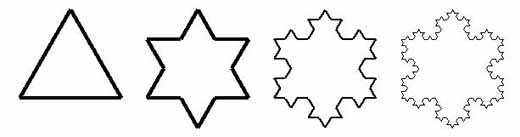
\includegraphics[width=9cm]{snowflake.jpg}
	\caption{The initial equilateral triangle and the refinement of the Koch
		snowflake after one, two, and three iterations.}
\end{figure}
an equilateral triangle and repeat the following an infinite number
of times:
\begin{quote}
\emph{Divide all line segments into three segments of equal length. Then draw,
	for each middle line segment, an equilateral triangle that has the middle
	segment as its base and points outward. Finally, remove all middle segments.
	}
\end{quote}
Figure 1 shows the first iterations in the construction.
%\marginpar{(Original)}
%
%
\subsection{Two properties}
\begin{theorem}
	The Koch snowflake has infinite length.
\end{theorem}
\begin{proof}
Let $\Delta$ denote a triangle, with side length $s$, on which
we base the construction of a snowflake. Let $N_i$ denote the number of line
segments, and $L_i$ the length of the segments, in iteration $i$ of the
construction. Then%
$$%
	N_n =
	\begin{cases}
		3 &\text{if } n = 0 \text{ (i.e.\ before any iterations), and} \\
		4N_{n-1} &\text{otherwise,}
	\end{cases}
$$%
which solves to
\begin{equation} \label{eq:first}
	N_n = 3 \cdot 4^n,
\end{equation}
while
\begin{equation}\label{eq:second}
	L_n = \frac {L_{n-1}} {3} \uberfrac{2} \uberfrac{3} = \ldots =
		\frac{L_0} {3^n} = \frac s {3^n}.
\end{equation}
From Eqs.~\ref{eq:first} and~\ref{eq:second}, the total length
$$
	N_nL_n = 3 \cdot 4^n \frac s {3^n} = 3s \frac {4^n} {3^n} = 3s \left (
		\frac 4 3
	\right )^n.
$$
Since $4/3 > 1$, it follows that $N_nL_n$ tends to infinity as
$n \to \infty$, i.e.\ the Koch snowflake has infinite length.
\end{proof}
\begin{theorem}
	The Koch snowflake has finite area.
\end{theorem}
\begin{proof}
In an iteration, a triangle is added on each line segment of the
previous iterations. So, in iteration $n$, the number of new triangles
$T_n = N_{n-1}$, which, by Eq.~\ref{eq:first}, can be simplified to
\begin{equation}\label{eq:third}
	T_n = \frac 3 4 \cdot 4^n.
\end{equation}
The area $a_n$ of each such triangle, with the exception of the area
$a_0 = \frac {\sqrt 3} 4 s^2$ of $\Delta$, is one ninth of the area of a
triangle added in iteration $n - 1$, or
%
\begin{equation}\label{eq:fourth}
	a_n = \frac {a_{n-1}} {9}
		= \frac {a_{n-2}} {9^2}
		= \frac {a_{n-3}} {9^3}
		= \ldots
		= \frac {a_0} {9^n}.
\end{equation}
This means that in iteration $n$, by Eqs.~\ref{eq:third} and~\ref{eq:fourth}, the area of all added
triangles
$$b_n = T_na_n = \left (
		\frac 3 4 \cdot 4^n
	\right )
	\left (
		\frac {a_0} {9^n}
	\right ) = \frac {3a_0} 4 \left (
	\frac 4 9
	\right )^n.$$
All in all, after iteration $n$, the total area
%\marginpar{(Original)}
\begin{align*}
	A_n &= a_0 + \ubersum{}{1} b_k \\
		&= a_0 \left (
				1 + \frac 3 4 \ubersum{}{1}\left(\frac 4 9 \right )^k
			\right ) \\
		&= a_0 \left (
				1 + \frac 1 3 \ubersum{-1}{0}\left(\frac 4 9 \right )^k
			\right ) \\
		&= a_0 \left (
				1 + \frac 3 5 \left ( 1 - \left( \frac 4 9 \right )^n \right )
			\right ) \\
		&= \frac {a_0} 5 \left (
				8 - 3 \left ( \frac 4 9 \right )^n
			\right ).
\end{align*}
Now, since
$$
	\lim_{n \to \infty} 3 \left ( \frac 4 9 \right )^n = 0,
$$
it follows that $\lim_{n \to \infty} A_n = \frac {8a_0} 5$, i.e.\ the Koch
snowflake has finite area.
\end{proof}
%\bibliography{theorem}{}
\begin{thebibliography}{99}
	\bibitem{aoeu}
		H. von Koch.
		\emph{Sur une courbe continue sans tangente, obtenue par une
		construction géométrique élémentaire}.,
		Arkiv för matematik, astronomi och fysik, Kungliga Vetenskapsakademien.
		{\bf 1},
		681-702,
		1904.
\end{thebibliography}

%\bibliographystyle{plain}

\end{document}
